\documentclass[sigconf,review]{acmart}

\usepackage{subcaption}
\usepackage{cleveref}

\crefname{figure}{Figure}{Figures}

\acmConference[SPLC'25]{29th International Systems and Software Product Line Conference}{September 01--September 05, 2025}{A Coruña, Spain}

\begin{document}

\title{On digital LEGO product lines for engineering education}

\author{Aleksandra Erohina}
\affiliation{
    \institution{University of Applied Sciences Upper Austria}
    \department{School of Engineering}
    \city{Wels}
    \state{Upper Austria}
    \country{Austria}
}

\author{Georg Hackenberg}
\orcid{0000-0003-3913-4148}
\affiliation{
    \institution{University of Applied Sciences Upper Austria}
    \department{School of Engineering}
    \city{Wels}
    \state{Upper Austria}
    \country{Austria}
}
\email{georg.hackenberg@fh-ooe.at}

\begin{abstract}
    TODO
\end{abstract}

\keywords{LEGO}

\maketitle

\section{Introduction}
\label{sec:introduction}

TODO~\cite{Hackenberg_2023} TODO~\cite{Baldwin_2023}

\paragraph{Research objective}

TODO

\paragraph{Research question}

Can we use digital LEGO for building interesting use cases for product line engineering that work well in engineering education?
Can we see typical issues in product line engineering such as module incompatibility in these use cases?
Can we use existing tools for digital LEGO modeling to build up relevant use cases already today?

\paragraph{Contribution}

TODO

\section{Related work}
\label{sec:related-work}

TODO

\section{Case study}
\label{sec:case-study}

In this third chapter we introduce the case study, which we have prepared for testing the viability of digital LEGO for product line engineering education.
In the following, we first provide an overview of the selected product line and its product variants in Section~\ref{sec:product-variants}.
Then, we introduce the atomic modules of the product line, from with the individual variants have been assembled in Section~\ref{sec:atomic-modules}.
Finally, we explain the configuration options of the drone use case in the form of a feature tree model in Section~\ref{sec:configuration-options}.

\subsection{Product variants}
\label{sec:product-variants}

\cref{fig:product-variants} provides an overview of the product variants for the drone use case.
The use case comprises three product variants, an ultra-light drone (see \cref{fig:ultra-light}), a free-style drone (see \cref{fig:free-style}), and a long-range drone (see \cref{fig:long-range}).

\begin{figure*}[htbp]
    \subcaptionbox{Ultra-light variant\label{fig:ultra-light}}{
        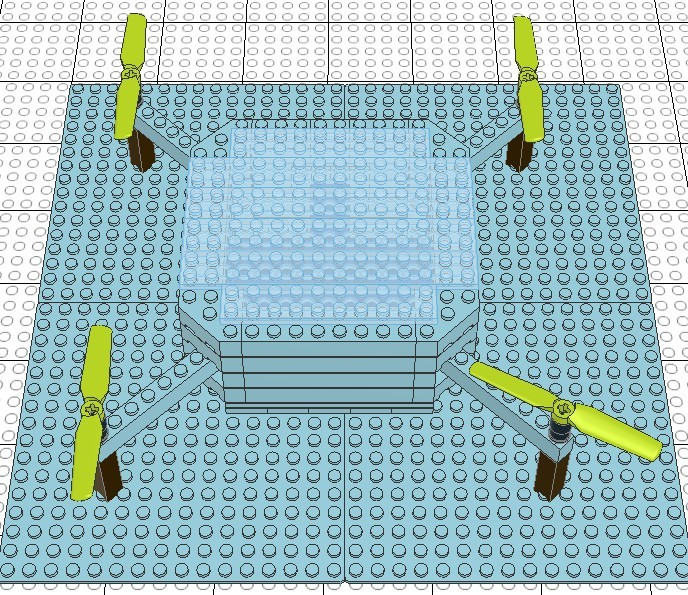
\includegraphics[height=4.4cm]{./drone-case-final-ultralight.jpg}
    }
    \hfill
    \subcaptionbox{Free-style variant\label{fig:free-style}}{
        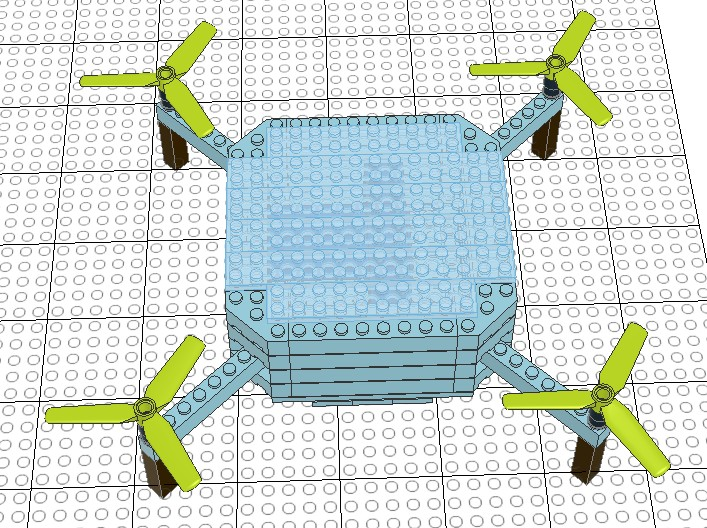
\includegraphics[height=4.4cm]{./drone-case-final-freestyle.jpg}
    }
    \hfill
    \subcaptionbox{Long-range variant\label{fig:long-range}}{
        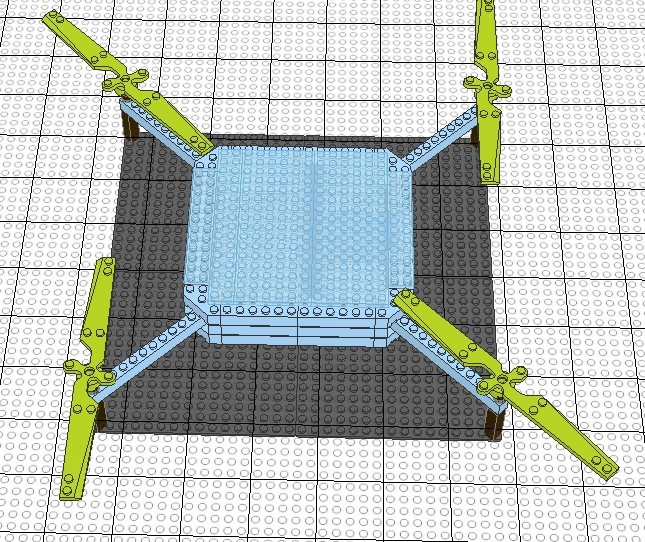
\includegraphics[height=4.4cm]{./drone-case-final-longrange.jpg}
    }
    \caption{Overview of the product variants for the drone use case.}
    \label{fig:product-variants}
\end{figure*}

\subsection{Atomic modules}
\label{sec:atomic-modules}

TODO

\begin{figure*}[htbp]
    \subcaptionbox{Small frame\label{fig:frame-small}}{
        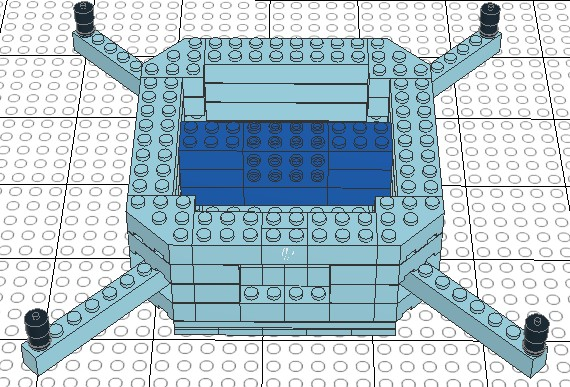
\includegraphics[height=2.3cm]{./drone-case-modules-frame-small.jpg}
    }
    \hfill
    \subcaptionbox{Large frame\label{fig:frame-large}}{
        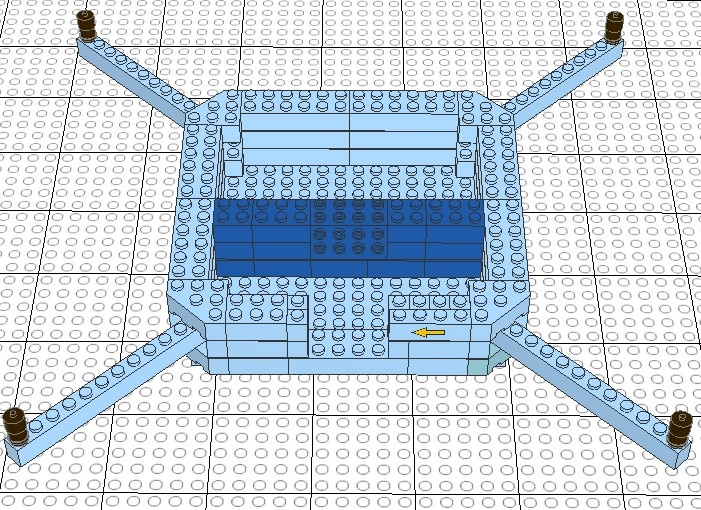
\includegraphics[height=2.3cm]{./drone-case-modules-frame-large.jpg}
    }
    \hfill
    \subcaptionbox{Small battery\label{fig:battery-small}}{
        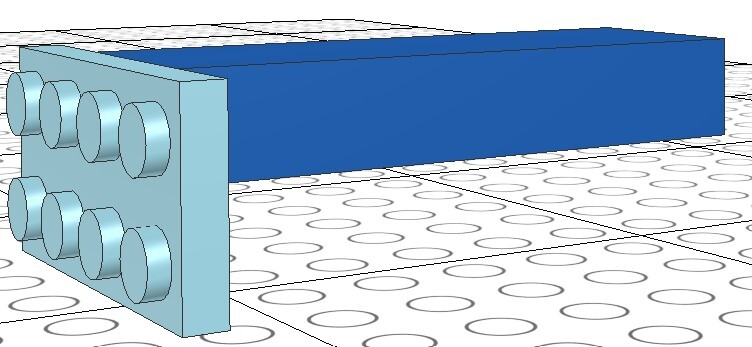
\includegraphics[height=1.3cm]{./drone-case-modules-battery-small.jpg}
    }
    \hfill
    \subcaptionbox{Medium battery\label{fig:battery-medium}}{
        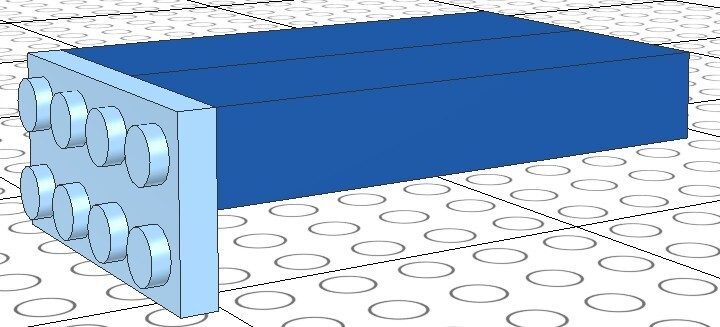
\includegraphics[height=1.3cm]{./drone-case-modules-battery-medium.jpg}
    }
    \hfill
    \subcaptionbox{Large battery\label{fig:battery-large}}{
        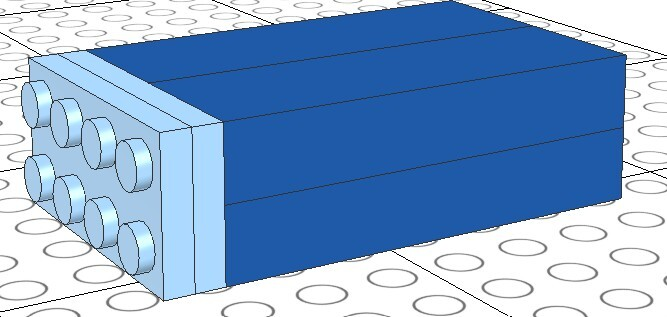
\includegraphics[height=1.3cm]{./drone-case-modules-battery-large.jpg}
    }
    
    \subcaptionbox{Small cover\label{fig:cover-small}}{
        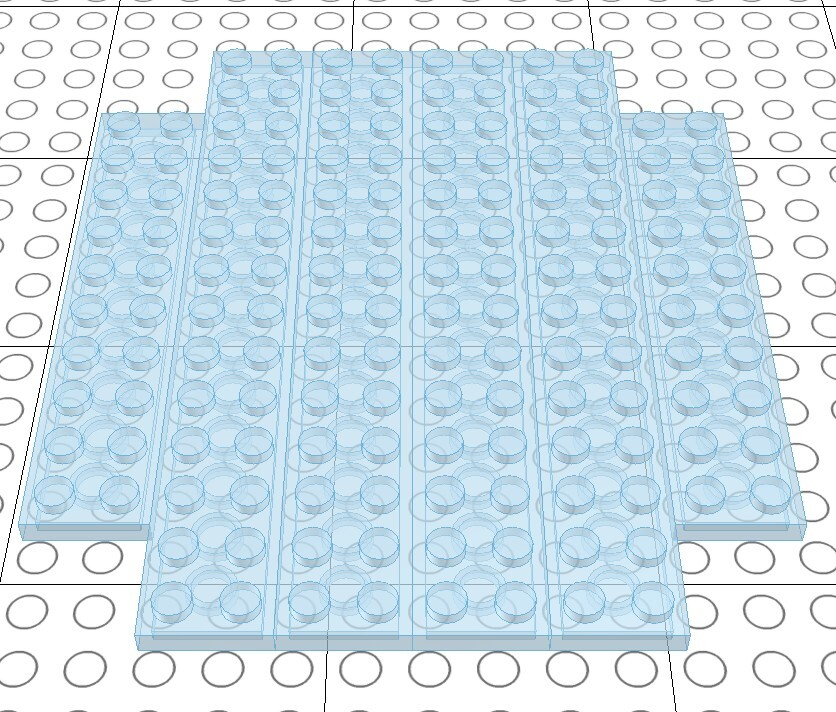
\includegraphics[height=2.3cm]{./drone-case-modules-cover-small.jpg}
    }
    \hfill
    \subcaptionbox{Large cover\label{fig:cover-large}}{
        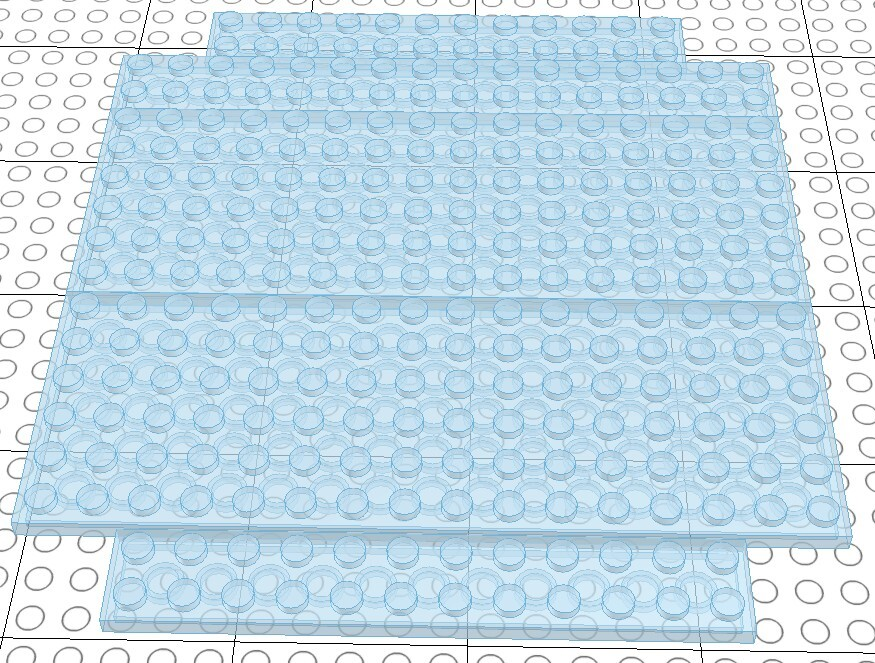
\includegraphics[height=2.3cm]{./drone-case-modules-cover-large.jpg}
    }
    \hfill
    \subcaptionbox{Small propellor\label{fig:propellor-small}}{
        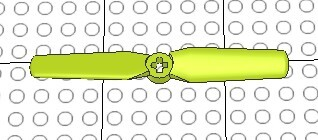
\includegraphics[height=1.5cm]{./drone-case-modules-propellor-2-small.jpg}
    }
    \hfill
    \subcaptionbox{Medium propellor\label{fig:propellor-medium}}{
        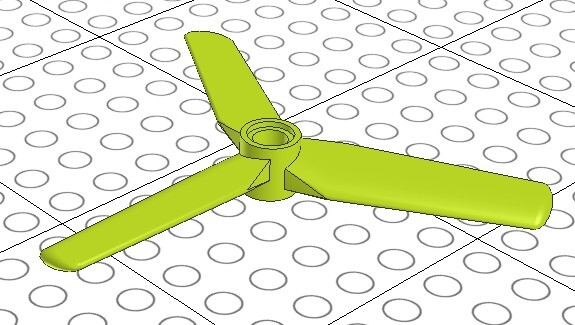
\includegraphics[height=1.5cm]{./drone-case-modules-propellor-3.jpg}
    }
    \hfill
    \subcaptionbox{Large propellor\label{fig:propellor-large}}{
        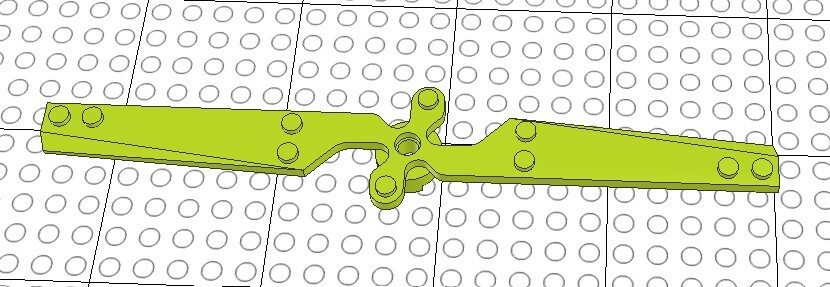
\includegraphics[height=1.5cm]{./drone-case-modules-propellor-2-large.jpg}
    }

    \caption{Overview of the atomic modules for the drone use case.}
    \label{fig:atomic-modules}
\end{figure*}

\subsubsection{Propellors}
\label{sec:propellors}

TODO

\subsubsection{Batteries}
\label{sec:batteries}

TODO

\subsubsection{Frames}
\label{sec:frames}

TODO

\subsubsection{Covers}
\label{sec:covers}

TODO

\subsection{Configuration options}
\label{sec:configuration-options}

TODO \cref{fig:feature-tree}

\begin{figure*}[htbp]
    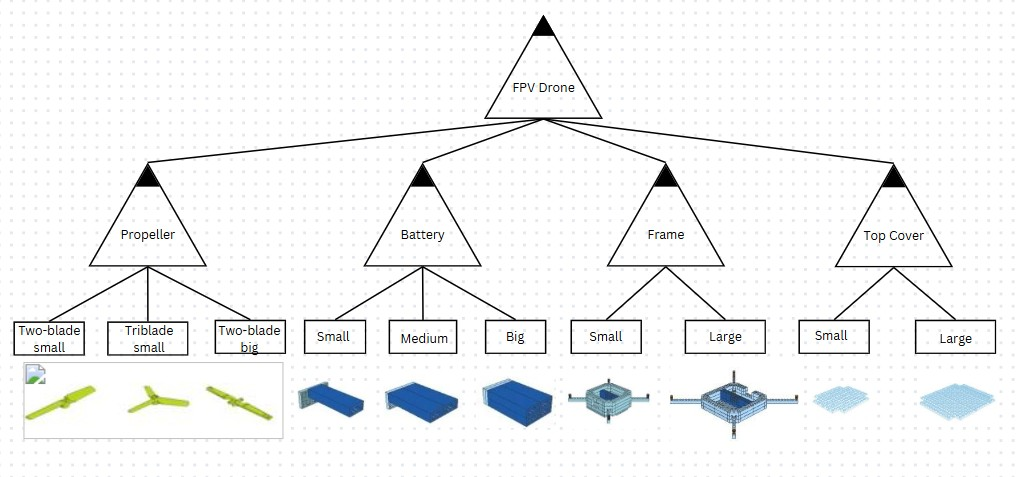
\includegraphics[width=\textwidth]{./drone-case-feature-tree.jpg}
    \caption{Overview of the configuration options for the drone use case.}
    \label{fig:feature-tree}
\end{figure*}

TODO

\section{Conclusion}
\label{sec:conclusion}

TODO

\bibliography{main}
\bibliographystyle{ACM-Reference-Format}

\end{document}